\section{New Architecture Designed with Using Our Metric}
\label{sec.newarchitecture}

Using our metric, we designed a new architecture to access the kernel in a more secure way. 

In this section, we describe the design and architecture of Lind. We explain the choices we made 
and the rationale behind our decision. We also discuss the challenges we are facing.

\subsection{Background}

In this section, we first discuss our threat model. We then give necessary description about 
the two sandboxing techniques that our work depends on. One is Google's Native Client sandbox, 
the other is Seattle's Repy sandbox. 

\subsubsection{Threat Model}

In our threat model, threats refer to any behavior that may cause potential harm to the system, 
which may be triggered by malicious code or bugs in non-malicious programs.

In order to fully execute their functions, applications need to have access to a set of privileges provided by 
the operating system, usually exposed as system calls. The primary security goal of a sandbox is to 
restrict a program to some subset of privileges, usually by exposing a set of functions that mediate 
access to the underlying operating system privileges. Threats occur when applications obtain access to 
privileges that were not intentionally exposed by the sandbox, thus escaping the sandbox \cite{Repy:10}.

To pose threats to a sandbox, we assume that applications may use multiple threads to modify visible state or issue concurrent requests which may trigger a race condition. Our goal is to prevent bugs in the code from 
allowing an user program to escape the sandbox.

\subsubsection{Google's Native Client Sandbox}

Google's Native Client (NaCl) is a sandbox for untrusted x86 native code \cite{NaCl:09}. 
NaCl aims to give applications the computational performance of native applications 
without compromising safety. NaCl uses software fault isolation 
and a secure runtime to direct system interaction and side effects through interfaces managed by NaCl. NaCl provides operating system portability for binary code while supporting performance-oriented features, 
such as thread support, instruction set extensions such as SSE, and use of compiler intrinsics and 
hand-coded assembler. 

We leverage NaCl execution environment. NaCl allows the efficient execution of legacy code 
in the form of x86 and ARM binaries that are built with a lightly modified compiler tool chain.

\subsubsection{Seattle's Repy Sandbox}

Seattle's Repy is a restricted subset of Python \cite{Repy:10}, which is a sandbox that 
provides safe environment for running applications.

In Lind, we use Repy to safely re-implement a subset of the POSIX API, which provides 
fundamental operating system access to many applications. The POSIX API, which itself is difficult to secure, 
is constructed using the Seattle's Repy sandbox which provides performance isolation and safety. 


\subsection{Our New Design}

The primary goal of Lind is to execute untrusted applications in a secure way. To achieve this goal, 
we try to minimize the portion of reachable kernel which might be exposed to applications in the user space. 
Existing system call interface in the kernel is rich and exploitable. We decided to safely re-implement most OS
functionalities in our Repy sandbox. We use Repy sandbox to reconstruct a POSIX interface, which provides 
OS functionalities sufficient for most applications. 
   
When security goal is achieved, we still want to execute applications efficiently, preferably in a light-weight 
way that can reduce potential overhead. We leverage Google's Native Client (NaCl) to achieve
this second goal of efficiency.  

Combining both NaCl and Repy sandbox, we have formed our dual-layer sandbox architecture 
design of Lind. (Shown in Figure 2.)  


\begin{figure}[h]
\centering
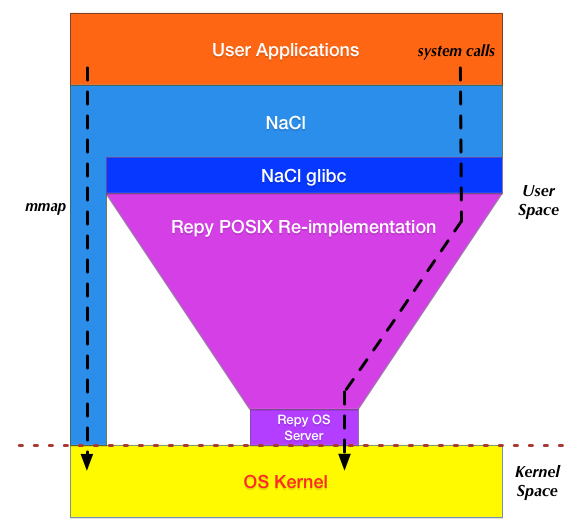
\includegraphics[width=1.0\columnwidth]{diagram/lind_architecture.png}
\caption{Architecture of Lind}
\label{fig:arch}
\end{figure}


To provide native computation and safe access to the system, Lind combines NaCl and Repy. 
Untrusted programs are run in NaCl, but access to all system resources is diverted to our Repy program. 
This program is responsible for accessing the system on behalf of the program, it is called the Lind Library OS. 
Our NaCl sandbox is built on top of our Repy sandbox. To service a system call in NaCl, a server routine 
marshals its arguments into a text string, and sends the call and the arguments to Repy sandbox. 
The Library OS then executes the appropriate system call, marshals the result and returns it back to NaCl. 
The result is eventually returned as the appropriate native type to the calling program. 

Lind is designed to minimize its footprint within the trusted code base (TCB) of these two sandboxes. 
To achieve that, most of the Lind code is run from within the two sandboxes, the modifications to 
the sandboxes themselves (and therefore the TCB) was extremely small. 

The dual-layer sandbox mechanism completes the achievement of the isolation design goals through 
two features. First, the dual-layer sandbox ensures that all code can modify only device state, 
interact with devices, or interact with the outside world through the new trusted operating system interface. 
Secondly, the customizability of the interface ensures that the system can only modify state, interact with 
devices, or interact with the world at a rate and in a manner specified for the application. For example, 
any attempt to send spam or execute a denial of service attack would trigger limits on resource 
consumption and/or allowable addressing, and would be prevented. 

The dual-layer sandbox also makes the construction of Lind simpler. The complex part of Lind is the 
Library OS which runs in Repy. However, Python is a very powerful language, so it significantly simplified 
the construction of Lind. Even though Python is considered ``slow'' by some, the internals of 
an application in Lind are run in NaCl, a very high performance environment. 
This balances the performance of the system, with the ease of implementation and maintenance 
of the Library OS component of Lind. 

Furthermore, this particular design and architecture for sandboxing ensures the programs are portable. 
Programs running inside Lind are written to work against a standard POSIX glibc interface. 
The Lind runtime is strictly user-level and designed to work on many different platforms including Linux, 
Mac OS X and Windows.

Our sandbox also ensures performance isolation. It is used to limit resource consumption, 
both of computational resources (CPU, memory) and external resources (disk I/O and space, 
network bandwidth). The interposed system calls rate limit access and total consumption of 
each class of device on a configurable basis. CPU and memory limits are enforced on 
a per-process basis. 

Finally, this kind of sandboxing ensures that the lightweight goal is met. Overhead for the Lind system 
is low because the sandbox only incurs overhead when there is a system call; Lind uses a native interface 
for execution, allowing CPU-and-memory-intensive applications to run at speeds that are equivalent 
to NaCl and near native speed. 

Regarding our dual-layer sandbox architecture, one fundamental question is: are two sandboxes 
enough and necessary? Why do we only have two sandboxes? If sandboxing provides more security, 
why not sandbox Repy sandbox's TCB and get more security? The answer to that question is: 
the lowest level sandbox eventually must have some fundamental yet limited access to system resources, 
such as memory, storage, threads, etc. So having multiple sandboxes is not necessary, and two sandboxes in 
our design would be enough. But are two sandboxes indeed necessary? Why not just have one sandbox 
that solves everything? The answer is that the kernel interface is extremely rich and hard to protect. 
In order to have minimal tough into the kernel, as well as provide sufficient API for legacy applications, 
we need to have more than one sandbox to complete the job. One sandbox focuses on protecting 
the kernel and providing POSIX API, the other sandbox deals with executing applications efficiently. 
That is the reason for us to have at least two sandboxes.  

The key point in our design is to achieve safe re-implementation of OS functionalities. 
However, our safe re-implementation has limitations. There are a few functionalities that 
we currently cannot re-implement in our sandbox. Those functionalities include brk, mmap, and threads creation.